\documentclass[12pt, letterpaper]{article}

% Imports
\usepackage{fancyhdr}
\usepackage{pgfplots}
\usepackage{geometry}
\usepackage{icomma}
\usepackage{amsmath}
\usepackage{multicol}
\usepackage{mathptmx}
\usepackage{anyfontsize}
\usepackage{t1enc}
\usepackage{tabto}
\usepackage{listings}
\usepackage{filecontents}
\usepackage{subcaption}
\usepackage{tikz}
\usepackage[parfill]{parskip}
\usepackage{graphicx}
\usepackage[]{mdframed}
\usepackage{amsmath}
\usepackage[makeroom]{cancel}
\pgfplotsset{compat=1.18}
\usepackage{tkz-euclide}
\usepackage{siunitx}
\sisetup{quotient-mode=fraction} % Output a/b as \frac{a}{b}

\geometry{margin=2.5cm}

\newcommand{\name}{Kaleb Burris}
\newcommand{\classname}{PHYS 211X}
\newcommand{\assignment}{FILL IN THE ASSIGNMENT}

\pagestyle{fancy}

\fancyhead[L]{
    \name 
    \newline
    \classname
    \newline
    \assignment
}

\newcommand{\horizontal}{\noindent\rule{\hsize}{0.4pt}}

\setlength{\headheight}{42pt}
\setlength{\headsep}{0.25in}
\setlength{\columnsep}{0.35cm}
\setlength{\columnseprule}{1pt}


\graphicspath{ {./lab10images/} }

% Put class number, class name, and professor 
% name.
% Use only in case of emergency, this
% should be covered by the preamble.
% \renewcommand\classname{}

% Put the assignment name with \S if 
% necessary for the section and the question 
% numbers.
\renewcommand\assignment{Lab 10, Day 2: An exploration and discussion of Natural Frequency and Resonance, 3/28/2023, Partners: Maite Valentin-Lugo, Seth Waln}

\begin{document}

    % Templates
    \iffalse
    % Use these for equations.
    \begin{equation*}
        \begin{gathered}
            Equations go here.
        \end{gathered}
    \end{equation*}

    % Use this if a line of math is too long.
    \resizebox{\hsize}{!}{$Long equation goes here$}

    % Use these for multiple columns.
    \begin{multicol*}{# of columns}
        % Remove the * if you want the columns to be balanced.
    \end{multicol*}

    % Use this to add a horizontal line.
    \horizontal

    \fi

    % Begin homework here.
    %%%%%%%%%%%%%%%%%%%%%%

    \section*{Station 1: Elastic Band}

    \begin{itemize}
        \item [1.]\mbox{}
        
        \begin{center}
            Driving Frequency: 50Hz
    
            \begin{tabular}{| c | c |}
                \hline
                Tension & Antinodes             \\
                \hline
                0.8&7\\
                \hline
                1.0&6\\
                \hline
                1.2&5\\
                \hline
                1.4&5\\
                \hline
                1.6&4\\
                \hline
                1.8&4\\
                \hline
            \end{tabular}        
        \end{center}

        \item [2.]\mbox{}
        
        \begin{center}
            Tension: 1N
    
            \begin{tabular}{| c | c |}
                \hline
                Driving Frequency & Antinodes   \\
                \hline
                23&3\\
                \hline
                31&4\\
                \hline
                39&5\\
                \hline
                44&6\\
                \hline
                51&6\\
                \hline
                59&6\\
                \hline
            \end{tabular}        
        \end{center}

        \item [3.]
        
        \begin{align*}
            v       
                & = \sqrt{\frac{T_{s}}{\mu}}        \\
            \lambda 
                & = \frac{v}{f}                     \\
            \lambda 
                & \propto \frac{1}{\#A}             \\
            \frac{v}{f} 
                & \propto \frac{1}{\#A}             \\
            \frac{\sqrt{\frac{T_{s}}{\mu}}}{f}
                & \propto \frac{1}{\#A}             \\
            \sqrt{\frac{T_{s}}{\mu}}
                & \propto \frac{f}{\#A}             \\
        \end{align*}

        \pagebreak

        \item [4.]\mbox{}
        
        {\centering\resizebox{0.8\hsize}{!}{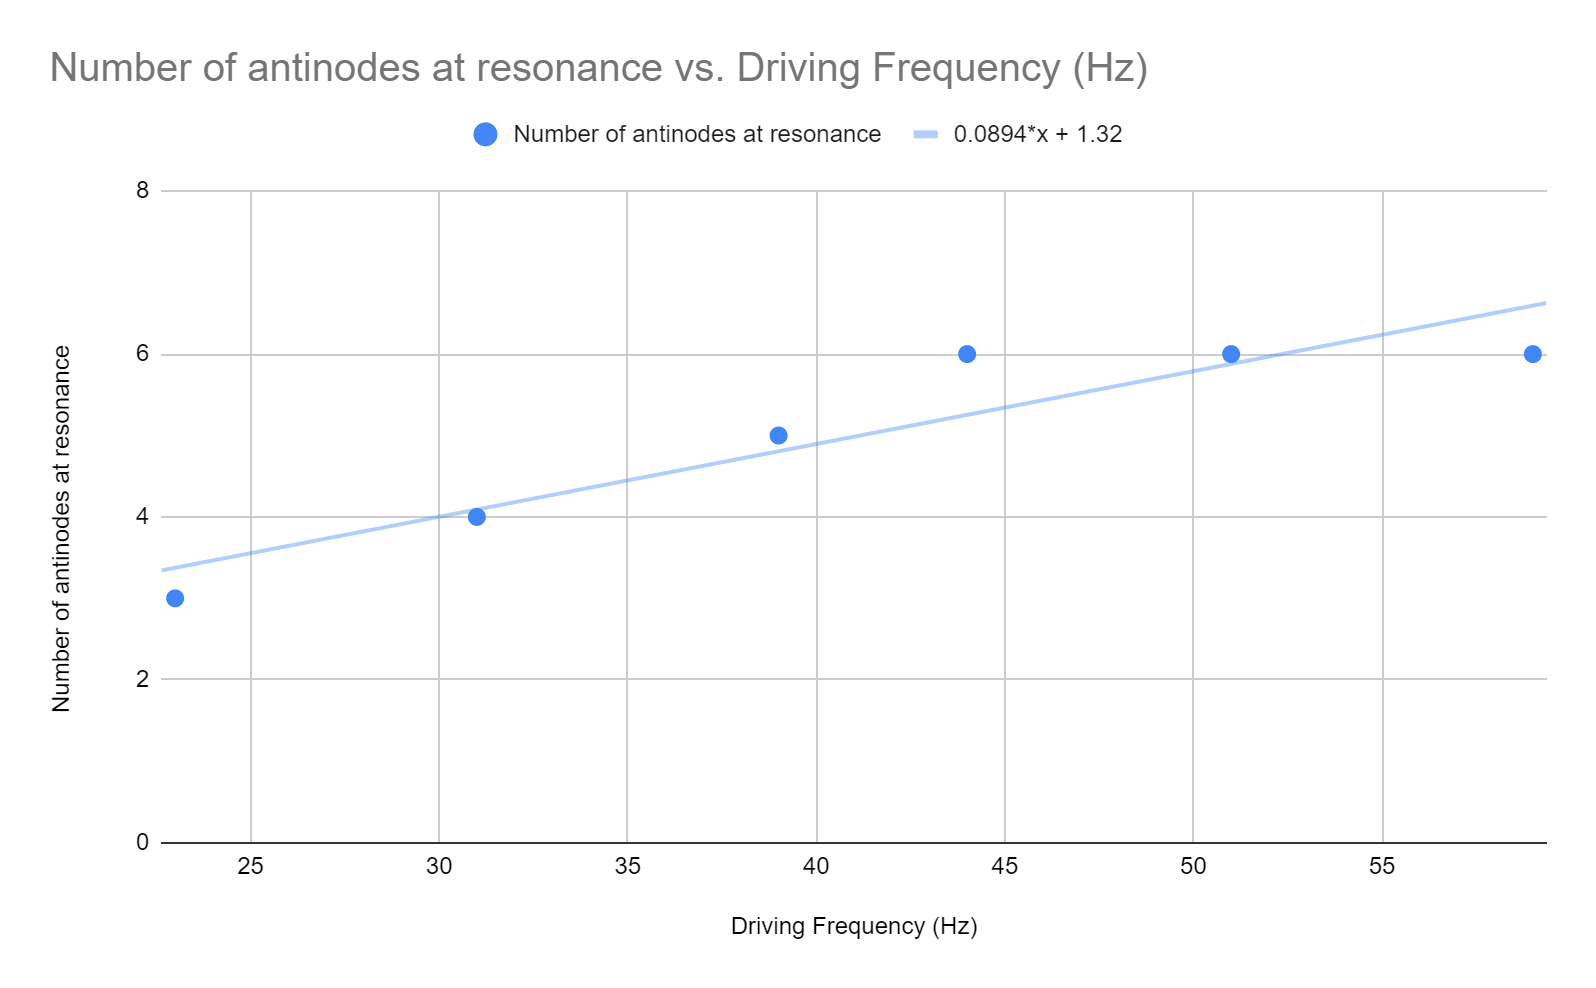
\includegraphics{image10}}}

        Our data closely matches the predicted result of following a linear relationship, although it started to deviate past 40 Hz.
        \item [5.]\mbox{}
        
        {\centering\resizebox{0.8\hsize}{!}{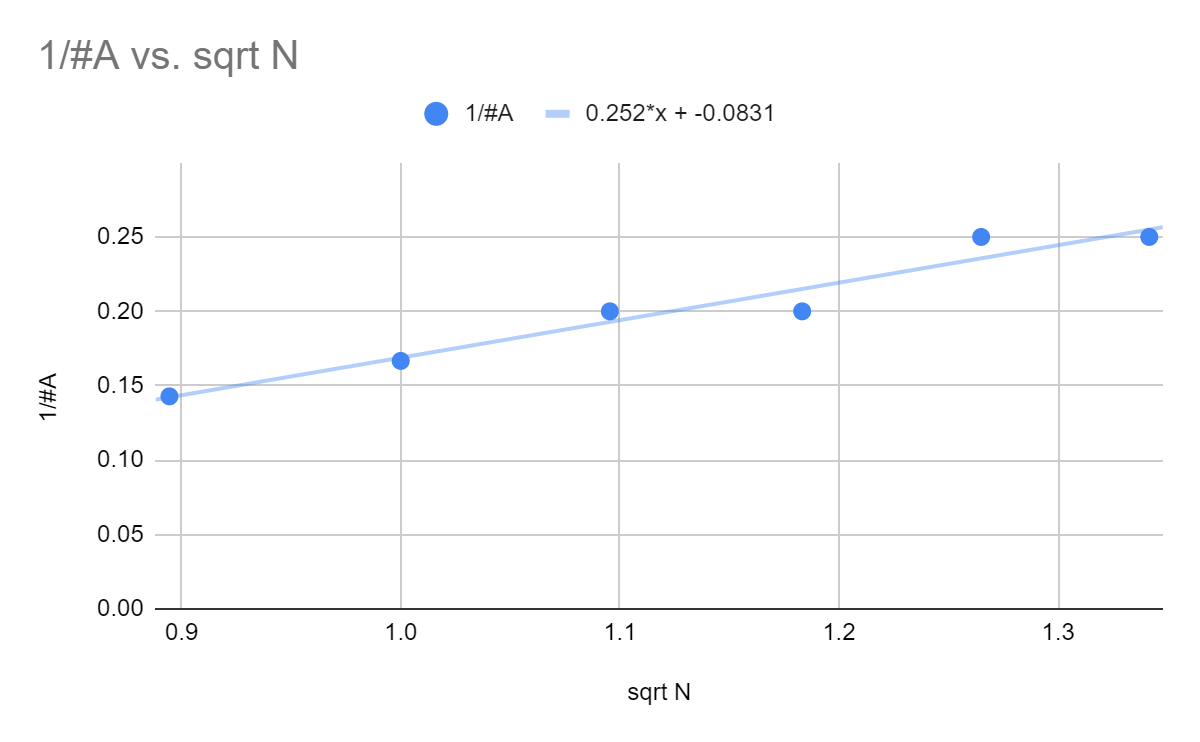
\includegraphics{image11}}}

        Our data very closely matched a linear regression, which tracks with the $\frac{1}{\#A}$ formula.

        \pagebreak
        
        \item [6.]\mbox{}
        
        \begin{center}
            \begin{tabular}{|c|c|c|c|}
                \hline
                & Tube 1 & Tube 2 & Tube 3  \\
                \hline
                Resonant frequency & 20 KHz & 16 KHz & 13 KHz \\
                \hline
                2nd Harmonic & 39 KHz & 32 KHz & 25 KHz \\
                \hline
                3rd Harmonic & 60 KHz & 48 KHz & 38 KHz \\
                \hline
            \end{tabular}
        \end{center}

        \item [9.]
        
        \begin{align*}
            \lambda & = \frac{2L}{\#A} = \frac{v}{f}    \\
            f   & = \frac{\#Av}{2L} 
                = \frac{1(343m/s)}{2(1.265m)} 
                = 135.57 hz                             \\
                & \rightarrow \{13.5KHz, 27KHz, 40.5Khz\}
        \end{align*}

        \item [10.]\mbox{}
        
        Our prediction was relatively close, at worst it was $1 - \frac{38}{40.5} = 6.2\%$ off of the expected value, and at best was $1 - \frac{13}{13.5} = 3.7\%$ off of the expected value. This error is pretty acceptable given the rough nature of the materials we used.
        
        \item[11.]\mbox{}
        
        \begin{center}
            \begin{tabular}{|c|c|c|c|c|}
                \hline
                & Attached Mass & Resonant Frequency & Natural Frequency & \% Difference    \\
                \hline
                Stiff Spring & 0.002 & 2.56 & 3.106 & 17.6\% \\
                \hline
                Medium Spring & 0.002 & 1.84 & 1.873 & 1.8\% \\
                \hline
                Soft Spring & 0.002 & 1.19 & 1.259 & 5.5\% \\
                \hline
            \end{tabular}
        \end{center}

        \item [12.]
        
        \begin{align*}
            \sqrt{\frac{70g}{50g}}    & = 1.18    \\
            1.18 \cdot 2.56 Hz       & = 3.02 Hz
        \end{align*}

        Real: 1.49 Hz, which is half of the predicted. We must have missed the first harmonic and got the second when we recorded.

        \item [13.] Our prediction was relatively good, but we missed the first harmonic. Scaling the prediction down, we would expect 1.56Hz, which is $1 - \frac{1.49}{1.56} = 4.5\%$ off of our prediction, which is pretty good and on track with the differences we've found experimentally thus far.
        
        \item [14.] The resonant frequency and natural frequencies we encountered seemed to be highly related in a 1:1 relationship with one another.
        
        \item [15.] \mbox{}
        
        \begin{center}
            \resizebox{\textwidth}{!}{\begin{tabular}{|c | c | c | c|}
                \hline
                & Natural Frequency Depends on: & How we drive the system: & At resonance observed, an increase in: \\
                \hline
                Elastic band & tension & Variable frequency mechanical oscillator & antinodes \\
                \hline
                Air column & length & Variable frequency speaker & amplitude \\
                \hline
                Mass on a Spring & Spring constant and mass & Variable frequency mechanical oscillator & amplitude \\
                \hline
            \end{tabular}}
        \end{center}

    \end{itemize}
    

\end{document}